%%
%%  Department of Electrical, Electronic and Computer Engineering.
%%  EPR400/2 Final Report - Section 3.
%%  Copyright (C) 2011-2018 University of Pretoria.
%%

\section{Design and implementation}


\subsection{Theoretical analysis}

The project was divided into two interfaces that would be integrated after they were complete to produce the final device. These were the handwriting recognition process and the communication process.

The handwriting recognition process required the analysis and understanding of natural language processing and machine learning. Computers gain the ability to make decisions based on calculations done by the use of machine learning. Machine learning involves the use of neural networks and statistical approaches like Hidden Markov Models.

When neural networks are used, computers have the ability to learn through implementations of algorithms that make use of these neural networks. A neural network is modelled after the human brain which has billions of neurons. Each of these neurons is connected to thousands of other neurons and these neurons exercise extensive parallel processing, helping the human brain detect information and make decisions in a very short burst of time. In the case of handwriting, a person sees a handwriting and then detects the words written. This may seem like a short trivial process, but a lot of processes are involved in the process. A picture of the handwritten word is passed to the brain. The brain feeds the information from the image to its neurons. Before this image is obtained however, the human must have learned about the characters in the alphabet and many patterns that they come in. The brain is trained with previous data to detect the characters in the word. For unrecognizable characters, the brain uses common sense to detect the most likely character to form a full word that makes sense. 

Neural networks do not work the exact same way, but they make use of the most important part of the brain, learning. A neural network that works close to the human brain contains millions of artificial neurons inter-connected to each other. When the cumulative input to a single neuron exceeds a certain threshold value, the neuron changes from an off state to an on state. The activation output is transmitted to other neurons that depend on this neuron. Because of neural networks’ capability to learn, they can generalize data well. When trained well enough, a neural network can find solutions to unseen data that is not part of the training set. In the scope of the project, the neural network should therefore be able to generalize for unseen handwriting inputs that are not part of the training set. This unseen handwriting will be known as the test set and this test set will be compared with the expected text output to find the accuracy of the neural network implemented. An important consideration is that the unseen data input should be under conditions similar to the training data therefore it is important for the unseen data to be noise-free. 

To incorporate the parallel processing property of the human brain into the neural network, the 100-step rule is applied. The human brain typically recognizes familiar objects in approximately 100 ms. The neuron switching time is approximately 1 ms. The number of time steps of parallel processing associated with the brain are equal to:

\begin{align*}
	\text{Number of steps} &=  \frac{\text{Recognition time}}{\text{Switching time}}\\
	 &=  \frac{100\text{ ms}}{1\text{ ms}}\\
	 &= 100 \text{ steps}
\end{align*}

	This corresponds to 100 assembler steps and it is not feasible for a computer using the 100-step rule to do anything. Therefore, the limitation is that neural networks cannot work as well as the human brain but can be modelled after it.

To get an accurate foundation of how neural networks work, the human brain is first analysed. The part of the body that processes information is called the vertebrate nervous system [11]. This system has a central nervous system which consists of the brain and the spinal cord. The rest of the human body’s nerves are part of the peripheral nervous system. Since the neural network model resembles the brain the central nervous system was looked at more closely.

The central nervous system acts as the CPU of the human body. The CNS manages all the information in the body. The brain is the important component to be analysed for the model to be designed. Within the brain are billions of information processing cells called neurons [12]. The trivial definition of a neuron is that it is a switch with an input and output. Multiple neurons contribute to the input of each neuron and if the sum of these neuron inputs is greater than a certain threshold, the switch is activated. \\
\begin{figure}[h]
	\centering
	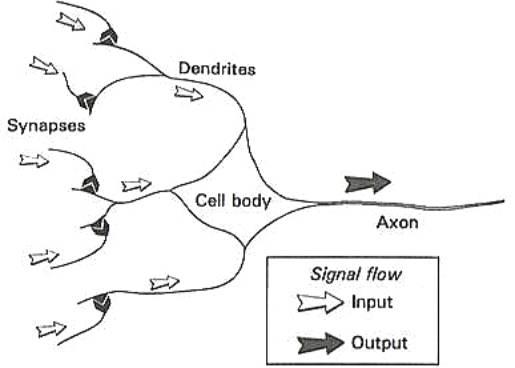
\includegraphics[scale=0.6]{4}
	\caption{Visual representation of a biological neuron}
\end{figure}

	Synapses receive the signals from the input neurons connected to that particular neuron. When a signal is received by the synapse, it is directly transmitted to the nucleus of the neuron. Dendrites receive the synapses that carry the signals from the input neurons and carry them to the nucleus of the neuron. The neuron’s nucleus sums up the inputs from the dendrites and when the summation exceeds a certain threshold value [13], an electrical pulse is activated. The neuron’s axon then transmits this pulse to the neurons whose inputs are connected to this neuron. Approximately 100 billion neurons are found in the human body.

The computer system executing the handwriting recognition process will model the biological neurons using artificial neurons. Artificial neurons are mathematical functions modelled after biological neurons to assist computers in learning like the human brain does. 

\begin{figure}[h]
	\centering
	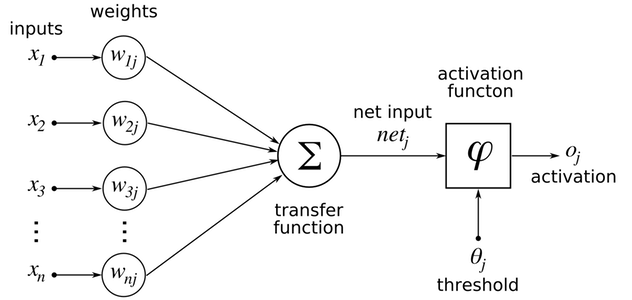
\includegraphics[scale=0.6]{5}
	\caption{Visual representation of an artificial neural network}
\end{figure}

An artificial neural network containing a single neuron layer is known as a perceptron. The perceptron takes vectoral input. This is information from neurons connecting to the input of the artificial neuron. In Figure 5, the inputs are the x values. These are typically contained in an array. They are represented as follows:
\begin{equation}
\text{Inputs}: \vec{x}= [x_1,x_2,x_3,x_4,..., ..., x_n]
\end{equation}

The vectorized inputs undergo a pre-processing phase where they are multiplied one-to-one with the vectoral weight components. The weights enable the perceptron to make conclusions from the inputs, giving each input a measure of significance. A significant part of the knowledge of the whole neural network therefore lies in the weights. The weights are represented as follows:
	
\begin{equation}
\text{Weights}: \vec{w} = [w_1j,w_2j,w_3j,w_4j,………,w_nj]
\end{equation}

The transfer function sums up the products of the inputs and their relevant significances to produce a single scalar value. This process is shown below:
\begin{align}
net_j &= x_1\cdot w_{1j}+ x_2\cdot w_{2j}+x_3\cdot w_{3j}+x_4\cdot w_{4j} \nonumber  \\
net_j &= \sum_{i=1}^j x_i \cdot w_{ij}
\end{align}

This value then undergoes a threshold test to determine if the neuron is switched on or off. This threshold test is known as an activation function. A trivial case of a simple threshold test is shown in the pseudo-code that follows.
		
\begin{algorithmic}
	\IF {$net_j > \phi$} 
	\STATE $\phi_j \leftarrow \textbf{ON}$
	\ELSE
	\STATE $\phi_j \leftarrow \textbf{ON}$
	\ENDIF 
\end{algorithmic}

In this case, if $net_j$ is greater than $\phi$ then the perceptron is activated by switching on its output while, if $net_j$ is less than $\phi$, the perceptron is not activated. The final output of the perceptron after the activation process is stored in $\phi_j$. The general activation function is represented by the symbol f and it calculates the exact value of $\phi_j$.

\begin{align}
\phi_j &= f(net_j) \nonumber\\
\phi_j &= f\big(\sum_{i=1}^j x_i \cdot w_{ij} \big)
\end{align}

An inter-connection of neurons is called an artificial neural network. A neural network is made up of neurons and weighted connections between them. The weighted connections transport output from the output of a neuron to the input of a dependent neuron. A simple example of a neural network is shown in the figure that follows.

\begin{figure}[h]
	\centering
	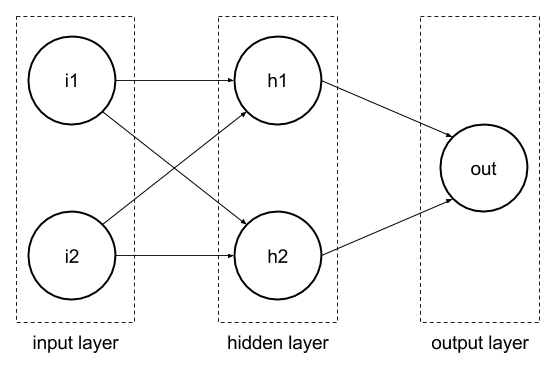
\includegraphics[scale=0.6]{66}
	\caption{Visual representation of a basic neural network}
\end{figure}

For the simple neural network in Figure 6, initial inputs i1 and i2 are weighted differently as they are passed to the hidden layers neurons h1 and h2. The i1 input to h1 is not necessarily the same as the i1 input to h2. This is because the connection to each of h1 and h2 is unique and independent to each other so the product of the weight and the scalar value from i1 is the input value to h1 or h2:

\hspace{20mm}i1 input to h1: $w_{i1-h1}\cdot i1$

\hspace{20mm}i1 input to h2: $w_{i1-h2}\cdot i1$

From the expressions above $w_{i1-h2}$ and $w_{i1-h1}$ are unique and different. The basic steps associated with any neuron in a neural network are shown in the figure below.

For a simple neural network, each neuron can be modelled to process data in the format shown in the diagram below.

\begin{figure}[h]
	\centering
	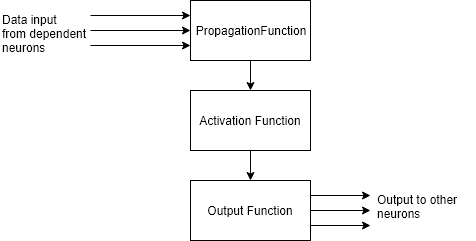
\includegraphics[scale=0.7]{7}
	\caption{Data processing functions in a neuron}
\end{figure}

The data input from each neuron is multiplied by the relevant weight to provide the input to the argument neuron. The propagation function is responsible for summing up the data inputs after different neurons after they have been multiplied by their relevant weights. These products are summed up to form a singular net input. The net input produced by the propagation function is passed to the activation function. The following mathematical functions describe the process associated with the propagation function.
	
Given a set of neurons, $I_s= \{i_1,i_2,i_3,…,…,i_n\}$ and the weight values for each neuron $w_{iz,j}$ are unique and independent ,and $z\, \varepsilon \, \{1,2,3,…,…,n\}$ , the cumulative network input to the neural network is calculated by the propagation function, $f_{prop}$ as follows:

\begin{align}
	net_j &= f_{prop} (\text{output}(I_s ),\text{weights to j}(w_{iz,j})) \nonumber \\  
net_j &=f_{prop} (o_{i_1},o_{i_2},o_{i_3} ,…,…,o_{i_n},w_{i1,j},w_{i2,j},w_{i3,j} )	
\end{align}

	
The input from each input neuron is the product of the weight to the argument neuron and the output from the input neuron. Therefore:

\begin{align}
	net_j = \sum_{i\, \varepsilon \, I} o_{i} \cdot w_{i,j}
\end{align}

The sum of these neuron inputs is shown in the equation above to be stored in $net_j$. This value of  $net_j$ is the value that is passed to the activation function in Figure 7. The activation function introduces non-linear properties to the network input. If an activation function were not to be used, the output would be a simple linear function whose polynomial degree is equal to 1. This type of polynomial has less ability to learn complex mappings. The activation is global for every neuron in the neural network and if the neural network has no activation function, it is known as a Linear Regression Model. A plot of this activation function is shown below:

\begin{figure}[h]
	\centering
	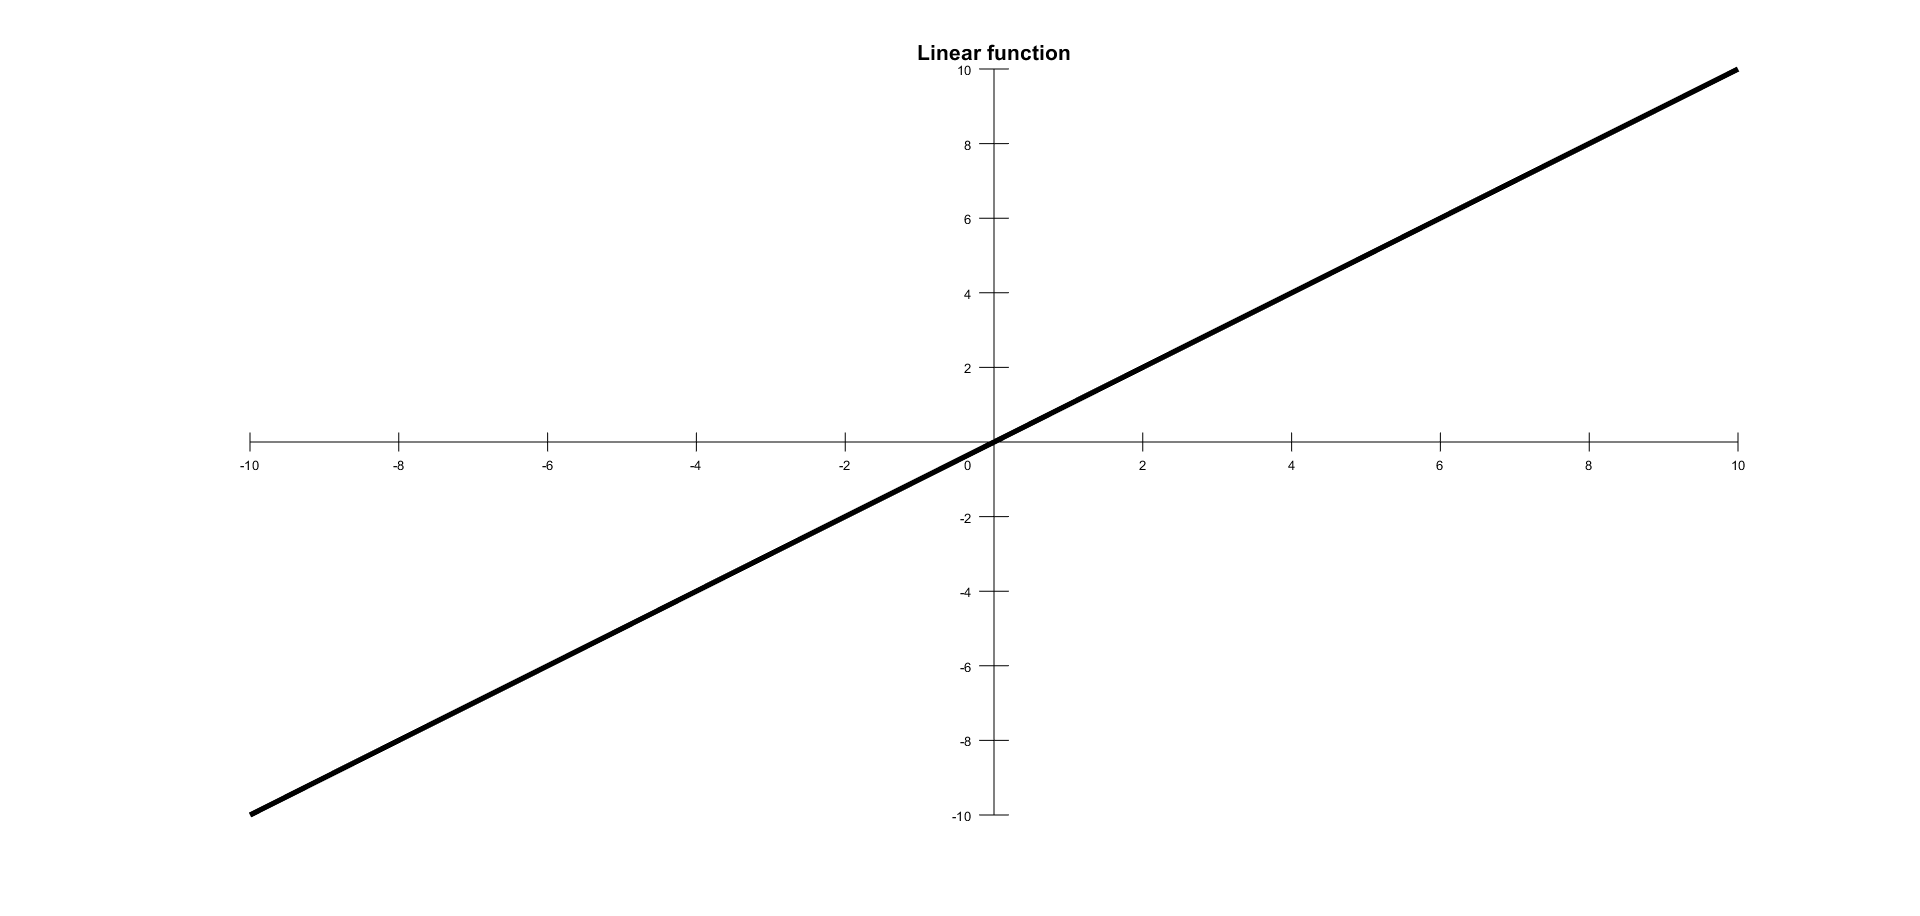
\includegraphics[scale=1]{8}
	\caption{Activation function for a Linear Regression Model}
\end{figure}

A neural network using a Linear Regression Model cannot properly model and learn from data inputs in the form of images, audio and videos. The output $a_j$ from this activation function, $f_{act}$ is given by:

\begin{align}
	a_j &= f_{act} (net_j) \nonumber \\
	a_j &= net_j
\end{align}

If instead a non-linear activation function is used, the result $a_j$ will be vastly different. The simplest non-linear activation function is the Heaviside function, which was defined in the introductory neuron example in the section. If the network input from passed from the propagation function is above a certain threshold, the activation function output changes from one value to another. If the value from the propagation function is less than the threshold value, the activation output remains the same. A plot of a binary threshold function is shown below.
\newpage
\begin{figure}[h]
	\centering
	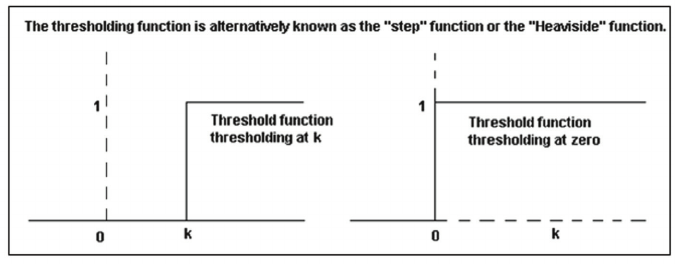
\includegraphics[scale=0.6]{9}
	\caption{Binary threshold function for k=0 and k$\neq$0}
\end{figure}

In this function, the x-axis values are the values from the propagation function, therefore the value of $a_j$ is calculated as follows:
\begin{gather*}
a_j :
\begin{cases}
	a_j = 1 & \text{for }net_j>k\\    
	a_j = 0 &  \text{for } net_j < k    
\end{cases}
\end{gather*}
It is important to note that the output values of $a_j$ do not necessarily have to be exactly 1 and 0 but they must be discrete and unique. As shown in the diagram, the values above and below the threshold are constant therefore their differential will be equal to zero since:
\begin{align}
		\frac{d}{d\,net_j} (a_j )&=\frac{d}{d\,net_j} (1)=  0 \quad \textbf{for} \quad net_j >k \\
		\frac{d}{d\,net_j} (a_j )&=\frac{d}{d\,net_j} (0)=  0 \quad \textbf{for} \quad net_j \leq k
\end{align}

The value of $a_j$ is undefined at $net_j=k$ and therefore is undifferentiable at this value. Due to this condition, it is impossible to implement the backpropagation learning scheme on a neural network using the Heaviside function as its activation function.

The discontinuity in the function also poses an important question. If all the initial input $x$ values are equal to 0 so that:
$$\vec{x} = [0,0,0,.....0]$$
Using equation (3.3):

\begin{align*}
	net_j &= \sum_{i=1}^n x_i \cdot w_i \\
	&= \sum_{i=1}^n (0) \cdot w_i\\
	&= 0 
\end{align*}

This result leads to a result $net_j = 0$. As shown in Figure 10, this result is at the transition point of the neuron being switched on for $k=0$. Most inputs are initiated to be vectors with zero values, so there is a risk situation that could arise. To avoid the situation where the net input is exactly equal to the threshold value of $k=0$, a bias input equal to 1 is appended to the inputs. This input will always be 1 and will also contain its own weight value. A representation of the new input system is shown below:

\begin{figure}[h]
	\centering
	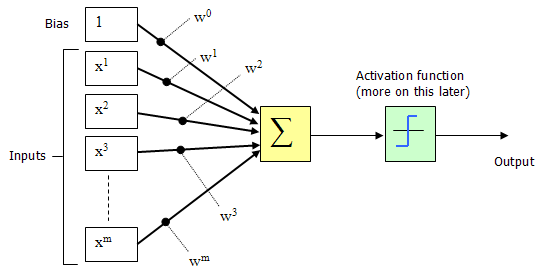
\includegraphics[scale=0.6]{29}
	\caption{Neural network with bias input}
\end{figure}

The above calculations apply primary to the Heaviside function with threshold $k=0$ which is the normally used activation function if a  Heaviside function is used. The equation to calculate the net input becomes:
\begin{equation}
	net_j = \big( \sum_{i=1}^m x_i \cdot w_i \big) + 1\cdot (w_o)
\end{equation}
When the inputs supplied are equal to a zero array therefore the value of $net_j$ can be calculated as follows:
\begin{align}
	net_j &= \big( \sum_{i=1}^m x_i \cdot w_i \big) + 1\cdot (w_o)\nonumber \\
	net_j &= \big( \sum_{i=1}^m (0) \cdot w_i \big) + 1\cdot (w_o)\nonumber\\
	net_j &= 1 \cdot (w_o) 
\end{align}

In the equation above, the weight $w_o$ will be the determining factor of $a_j$. If $w_o < 0 $, then $net_j <0$, therefore $a_j  = 0$ . If $w_o >0$, then $net_j > 0$, therefore $a_j = 0$. These conditions work for the Heaviside function with threshold $k=0$. The threshold $k\neq 0 $ is slightly complex for the inputs that lead to $net_j = k$ and adjusting them thus it is not commonly used. 

Alternatively, the logistical function can be used as the activation function. If this function is used, the activation output will be calculated as follows:
\begin{align}
a_j&=f_{prop} (net_j)\\
&=\frac{1}{1+e^{-net_j}}	
\end{align}

This function leads to results $0 \leq a_j\leq 1$. The logistical function is differentiable as shown below:

\begin{align}
	\frac{d}{d\,net_j} (a_j )&=\frac{d}{d\, net_j} \big( \frac{1}{1+e^{-net_j}}\big) \nonumber \\	
	&=\frac {d}{d\,net_j} (1+e^{-net_j } )^{-1} \nonumber \\
	&=e^{-net_j} (1+e^{-net_j }  )^{-2} \nonumber \\
	&=\frac{e^{-net_j }}{(1+e^{-net_j } )^2} 
\end{align}

The logistic function can also be also be used to approximate a binary threshold function. A representation of the logistic function was plotted using the Python programming language.

\begin{figure}[h]
	\centering
	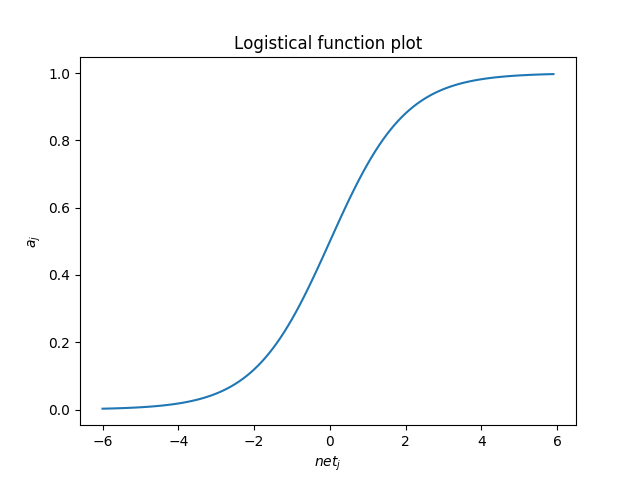
\includegraphics[scale=0.6]{10}
	\caption{Python plot for the logistic function}
\end{figure}

After the activation has been executed, the value of  $a_j$ is passed to the output function. The output function calculates the values to be distributed to the neurons whose inputs depend on this neuron’s output. For the neuron j, the output function of the neuron is:

\begin{equation}
	f_{out}=o_j	
\end{equation}

In the above equation, $o_j$ is the output of the output value of the neuron. Like the activation function, the output function is defined globally as well. In most cases, the output is the same as the value after the activation function:
\begin{align}
		f_{out}&=o_j \nonumber\\
	\text{But}\quad o_j&=a_j \nonumber\\
	\therefore f_{out}&=a_j
\end{align}

Different neural network topologies are analysed before making a choice on the correct implementation. Feedforward neural networks are the most trivial type of ANNs. The neurons that are in the network are divided into 3 layers. These layers are the input layer, the hidden layer and the output layer.

A plot of a simple feedforward neural network is shown below:
\begin{figure}[h]
	\centering
	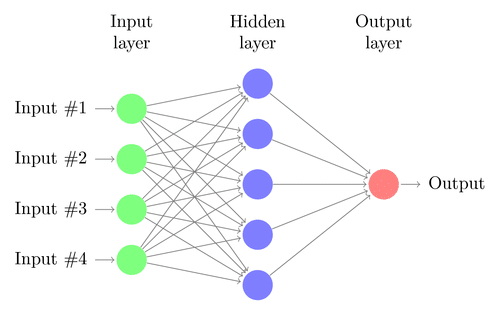
\includegraphics[scale=0.6]{11}
	\caption{Simple Neural Network with multiple input dependencies for each neuron}
\end{figure}

The neural network can have multiple hidden layers but only a single input layer as well as a single output layer. In this network topology, each layer’s neurons can only be directed to neurons in the next layer, thus the name feedforward network. Shortcut connections are possible for layers not immediately preceding the output layer to connect to the neurons at the output layer. A feedforward neural network works as follows: an input is supplied, and complex calculations are done on each neuron to produce final output values at the supposed output layer. However, there is an expected value associated with each input and the expected value is compared with the practical value output and the error associated with the result is calculated. This error is used to calculate the accuracy of the neural network.

There are different errors that can be used. Given output neurons are represented by $\Omega$ and the set representing output neurons is given by O, the specific error,$Err_p$ can be calculated by the equation:
\begin{equation}
	$\text { Err }$ _ { p } = \frac { 1 } { 2 } \sum_{ \Omega \in O }^{ }  \left( t _ { \Omega } - y _ { \Omega } \right) ^ { 2 }
\end{equation}

In the above neural network $t$ values are the true expected output values while $y$ values are the output values produced by the neural network. The Euclidean distance gives a more useful error value that the one calculated above as it will show how far the error correction has to be made to find the correct value. 
\begin{equation}
\operatorname {Err} _ { p } = \sqrt { \sum _ { \Omega \in O } \left( t _ { \Omega } - y _ { \Omega } \right) ^ { 2 } }
\end{equation}

The most desirable error is the root mean square error because it calculates the error values for the outlier outputs. This equation is shown below:
\begin{equation}
\operatorname { Err } _ { p } = \sqrt { \frac { \sum _ { \Omega \in O } \left( t _ { \Omega } - y _ { \Omega } \right) ^ { 2 } } { | O | } }
\end{equation}

The training of the neural network will follow an offline handwriting recognition scheme to minimize the learning time for the neural network. The outputs are batched and training occurs after a specific time period called an epoch. Epoch is an step in time where an expected value is calculated using feedforward propagation and the errors are corrected for weight adjustment for the dataset. The total error for each time interval of testing is important:

\begin{equation}
\text { Err } = \sum _ { p \in P } \operatorname { Err } _ { p }
\end{equation}

To be able to learn, the neural network uses a method called backpropagation where each neuron from the output back to the initial inputs has the weights of its inputs adjusted to minimize the error associated with the output. The gradient descent method is applied to the error. An example of the gradient descent is shown in the figure below:

\begin{figure}[h]
	\centering
	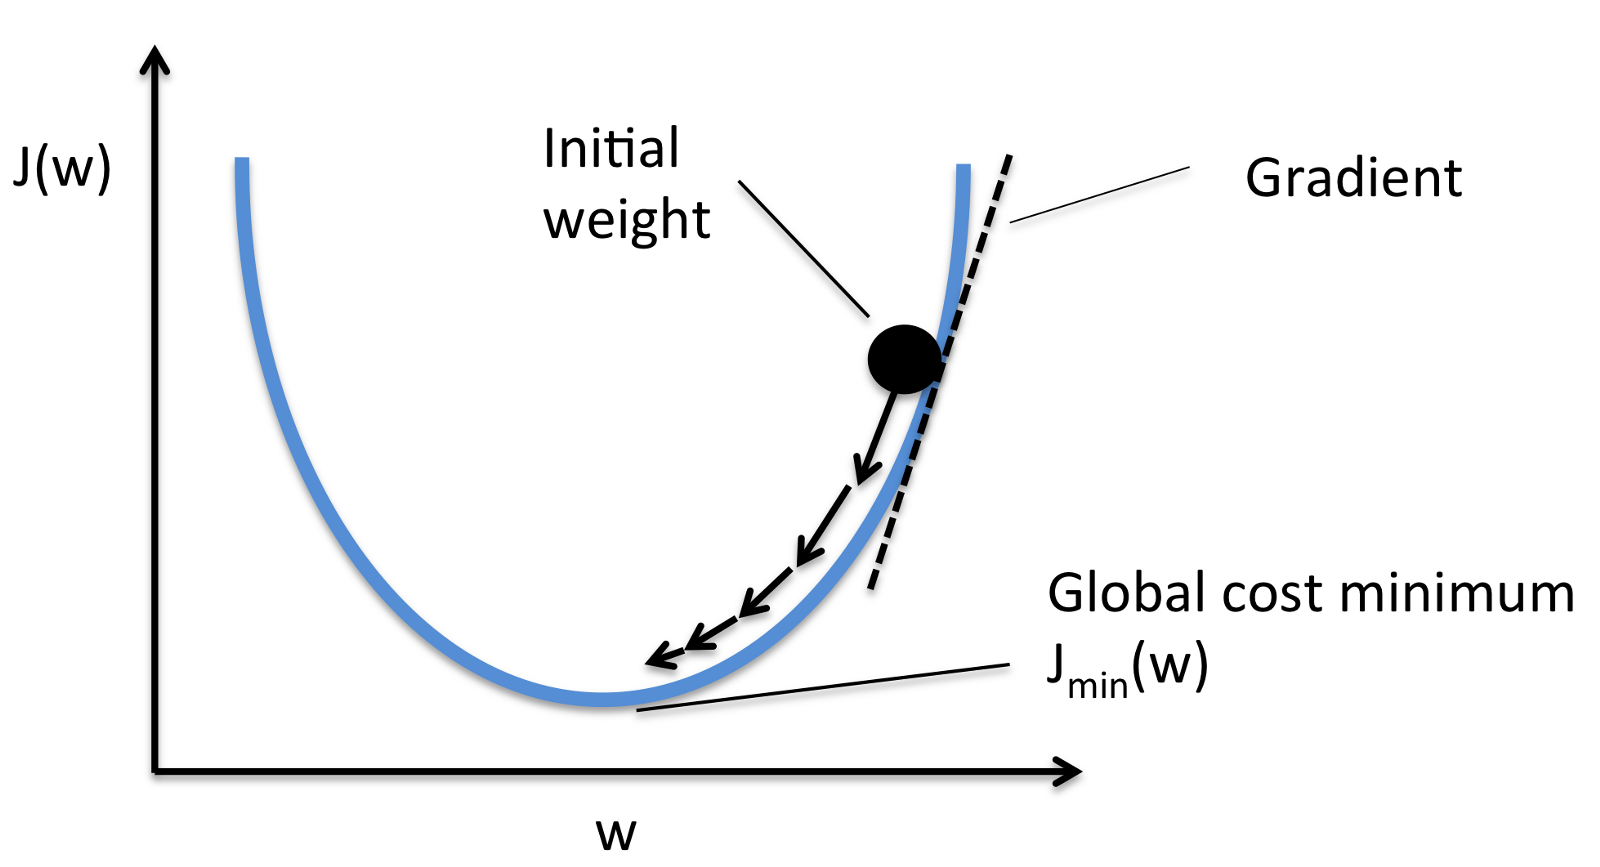
\includegraphics[scale=0.2]{31}
	\caption{Cost function example on which gradient descent can be applied.}
\end{figure}

The goal is to find a local minimum for each step so that the error is reduced to the minimum possible. The weight vector is gradually decreased, finding a new weight value that decreases the error function which is the cost function in the graph above. When the current position becomes the local minimum, instead of the one at the next step i.e. the net weight value increases the cost function instead of decreasing it, then mathematically the global minimum has been passed due to the step size being too large or the current value for the weight leads to the global minimum of the cost function. It is important to check the local minimum after every weight adjustment because continuous decrease without checking can overshoot the weight adjustment past the global minimum and weights end up a cost function that oscillates around the global cost minimum.

The neural network's learning function should model the figure that follows when  training data is supplied. The training data sample count does not have to be specific but the shape should follow or model the exponential curve. 

\begin{figure}[h]
	\centering
	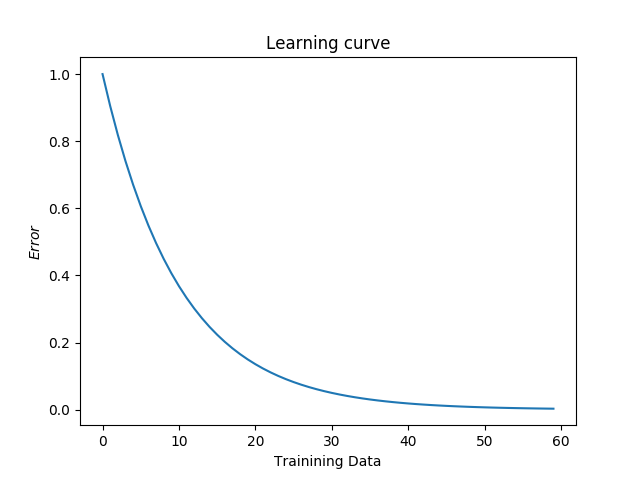
\includegraphics[scale=0.6]{30}
	\caption{Expected Learning curve for neural network}
\end{figure}

The value for adjusting the weights is directly proportional to the gradient of the cumulative Error.

\begin{align}
\Delta W \quad & \alpha \quad  \nabla \operatorname {Err} (W) \nonumber\\
\Delta W  &=  - \eta \nabla \operatorname { Err } ( W )
\end{align}
 
The constant $\eta$ is constant of proportionality known as the learning rate. It is equivalent to the step size of the weight adjustment. As described before, this value has to be optimized to avoid weight adjustments that lead to an oscillating error function. 

The gradient of the Error function is then expressed as the partial derivative with respect to the weights in the previous layer.
Every weight in the layer preceding the output layer is adjustment and the effect on the cumulative error function is analyzed. The adjustment follows the equation:

 \begin{equation}
 \Delta w _ { i , \Omega } = - \eta \frac { \partial \operatorname { Err } ( W ) } { \partial w _ { i , \Omega } }
  \end{equation}

The error function used for the weight adjustment is a combination of equation 3.17 and equation 3.19 so that:

\begin{align}
\text {Err}(W) &= \sum _ { p \in P } \operatorname { Err } _ { p }  \\
&= \sum_{p \in P} \big( \frac { 1 } { 2 } \sum _ { \Omega \in O } \left( t _ { \Omega } - y _ { \Omega } \right) ^ { 2 }\big)  \\
&=\frac{1}{2} \sum_{p \in P} \Big(  \sum _ { \Omega \in O } \left( t _ {p, \Omega } - y _ {p, \Omega } \right) ^ { 2 }\Big)
\end{align}

Equation 3.23 and 3.22 can be combined tp find the dependency of the weight ag=djustment on the individual errors:

\begin{align} 
	\Delta w _ { i , \Omega }  & = \sum _ { p \in P } - \eta \frac { \partial \operatorname { Err } _ { p } ( W ) } { \partial w _ { i , \Omega } } 
\end{align}

The partial derivative of each output's error function with respect to its weight is then calculated by using the chain rule so that the partial derivative of the error with respect to the ouput is multiplied by the partial derivative of the output with respect to the weight of that connection to the output.

\begin{equation}
\frac { \partial \operatorname { Err } _ { p } ( W ) } { \partial w _ { i , \Omega } } = \frac { \partial \operatorname { Err } _ { p } ( W ) } { \partial o _ { p , \Omega } } \cdot \frac { \partial o _ { p , \Omega } } { \partial w _ { i , \Omega } }
\end{equation}

The first argument of the equation in the chain rule can be broken down by first analyzing equation 3.17. This equation clearly shows that the error depends on the expected value of $t_{\Omega}$ and the observed value of $y_{\Omega}$. This value of $y_\Omega$ is the equivalent of the output value that is the derivative term i.e. $o_\Omega = y_\Omega$ as follows:
\begin{align}
\frac { \partial }{ \partial o _ { p , \Omega } }\Big(\operatorname { Err } _ { p } ( W )\Big) &= \frac { \partial }{ \partial o _ { p , \Omega } } \Big(\frac { 1 } { 2 } \sum _ { \Omega \in O } \left( t _ { \Omega } - o _ { \Omega } \right) ^ { 2 }\Big) \nonumber \\
&= (-1) \cdot 2 \cdot \frac{1}{2} \cdot (t_{p,\Omega} - o_{p,\Omega}) \nonumber \\
&= -(t_{p,\Omega} - o_{p,\Omega})
\end{align}

The specific error associated with the derivative can be replaced with a symbol $\delta_{p,\Omega} = t_{p, \Omega} - o_{p,\Omega}$. Equation 3.28 therefore becomes:
\begin{align}
\frac { \partial }{ \partial o _ { p , \Omega } }\Big(\operatorname { Err } _ { p } ( W )\Big) = -\delta_{p,\Omega}
\end{align}

Updating equation 3.27 leads to the equation:

\begin{align}
\frac { \partial \operatorname { Err } _ { p } ( W ) } { \partial w _ { i , \Omega } } &= \frac { \partial \operatorname { Err } _ { p } ( W ) } { \partial o _ { p , \Omega } } \cdot \frac { \partial o _ { p , \Omega } } { \partial w _ { i , \Omega } } \nonumber \\
 &= - \delta_{p,\Omega} \cdot \frac { \partial o _ { p , \Omega } } { \partial w _ { i , \Omega } }
\end{align}

For the derivative of the output with respect to the weight, it is realized that the output is the result after the activation process, which in turn depends on the net input as shown in equation 3.6 as this is a linear process as shown in Figure 9. This partial derivative reduces to:

\begin{align}
\frac { \partial o _ { p , \Omega } } { \partial w _ { i , \Omega } } &= \frac { \partial \sum _ { i \in I } \left( o _ { p , i } w _ { i , \Omega } \right) } { \partial w _ { i , \Omega } } \nonumber \\
\text{Therefore}\\
\frac { \partial \operatorname { Err } _ { p } ( W ) } { \partial w _ { i , \Omega } } &= - \delta _ { p , \Omega } \cdot \frac { \partial \sum _ { i \in I } \left( o _ { p , i } w _ { i , \Omega } \right) } { \partial w _ { i , \Omega } }
\end{align}

The above equation shows the summation of the outputs and th weights to destinations. However, all the derivatives are equal to 0 except for the term where the iterator $i=i$, sine they are constant with respect to $i$. The partial derivative of the output with respect to weight becomes:
\begin{align}
\frac { \partial o _ { p , \Omega } } { \partial w _ { i , \Omega } } &= \frac { \partial \sum _ { i \in I } \left( o _ { p , i } w _ { i , \Omega } \right) } { \partial w _ { i , \Omega } } \nonumber \\
&= \frac { \partial   \left( o _ { p , i } w _ { i , \Omega } \right) } { \partial w _ { i , \Omega } } \nonumber \\
&= o_{p,i}\\
\therefore \frac { \partial \operatorname { Err } _ { p } ( W ) } { \partial w _ { i , \Omega } } &= - \delta _ { p , \Omega } \cdot o_{p,i}
\end{align}

The equation (3.34) is inserted into the weight adjustment equation (3.26) to give the result:
\begin{align}
\Delta w _ { i , \Omega } &= \sum _ { p \in P } - \eta \frac { \partial \operatorname { Err } _ { p } ( W ) } { \partial w _ { i , \Omega } } \nonumber \\
&= \sum _ { p \in P } - \eta \cdot \big(- \delta _ { p , \Omega } \cdot o_{p,i}\big) \nonumber\\
&= \eta \sum _ { p \in P }   \delta _ { p , \Omega } \cdot o_{p,i}
\end{align}

The above equation will be the adjustment of the weight per epoch. To avoid the training time being too exponential, the training is done after every input which will be a screenshot of a line handwritten input. The equation then becomes:
\begin{align}
\Delta w _ { i , \Omega } &= \eta \cdot \delta _ { p , \Omega } \cdot o_{p,i}
\end{align}

Another type of neural network is the recurrent neural network. In general, for this type of network, each neuron contains a memory component that stores information about the previous input. In real life, when detecting a full sentence, the content of a word is dependent on the words detected before it. This type of neural network is therefore important in handwriting recognition. They are best applied to input that is only line segmented. A recurrent neural network works the same way as a feedforward network except the result for each input depends on the previous inputs. A recurring neural network consists of  multiple cascaded feedforward neural networks. The most important property of a recurring neural network is the presence of at least one feedback loop.

\begin{figure}[h]
	\centering
	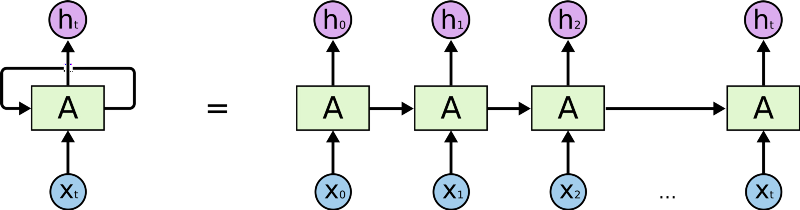
\includegraphics[scale=0.4]{12}
	\caption{Unfolding a Recurrent Neural Network}
\end{figure}

In the above example, for a time interval $t$, the $x_t$ values are the inputs, $A$ values are the neural network layers at time $t$ and $h_t$ values are the hidden state values at time $t$. The hidden state values from time $t-2$ or less are hidden from the state at time $t$ as it only has knowledge of the previous state. The output $h(t)$ is compared to the expected data output which is supplied in the test data. The error rate is calculated from this comparison and the backpropagation algorithm checks back to the previous layers of the neural network and adjusts the weights to minimize the error rate.\\
The present state can be summarized as being dependent on the current input and the parameters of the previous state:
\begin{align}
h _ { t } &= f _ { W } \left( h _ { t - 1 } , x _ { t } \right) \nonumber \\
h _ { t } &= \tanh \left( W _ { h h } h _ { t - 1 } + W _ { x h } x _ { t } \right)\nonumber\\
y _ { t } &= W _ { h y } h _ { t }
\end{align}

The equation above can be represented schematically by the diagram below:
\begin{figure}[h]
	\centering
	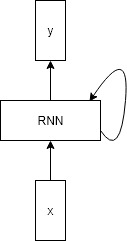
\includegraphics[scale=0.6]{15}
	\caption{Sketch showing the RNN process}
\end{figure}
\\
RNNs operate the same way as the previously described neural networks especially emphasizing on back propagation using the memory feature that they use. A problem arises where there is no stop condition due to the loop back being infinite and having no break condition. Learning could be done by unfolding the previous states of the RNN. The recurrences are backtracked, expanding the hidden states as shown in Figure 16. The earlier described backpropagation algorithm is applied to the unfolded Recurrent Neural Network. The weight values adjusted for RNNs from the backpropagation equations are the values of $W_{hh}$ and $W_{xh}$. Accuracy can be improved by expanding the non-output layers. The error associated with RNNs is dependent on the current and previous states i.e.
\begin{equation}
	Err_k = || \prod_{j=k+1}^{t} \frac{\partial h_j}{\partial h_{j-1}}||
\end{equation}

To prevent errors where the error associated with an input vanishes or disappears due to the exponential proportionality with time, Long Short Term Memory is used. Vanishing can occur if the product of the above equation keeps getting smaller with time while explosion occurs when the product exponentially increases.

The communication part of the device required the analysis of the GSM and well as the Wi-Fi method of communication. 
%If GSM were to be used for communication, the following diagram would model the architecture involved in the process.
\begin{figure}[h]
	\centering
	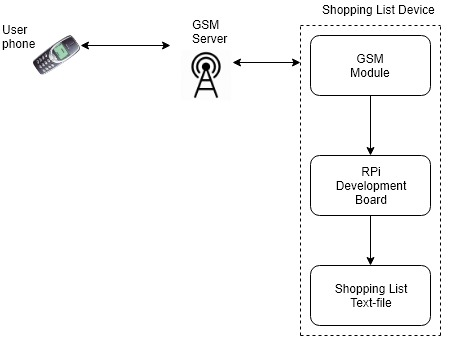
\includegraphics[scale=0.4]{17.jpg}
	\caption{Architecture involved in GSM communication}
\end{figure}

When GSM is used, mediums can communicate via voice or short message service or via fax. The operating frequencies of GSM communications are $450$ MHz, $800$ MHz, $900$ MHz, $1.8$ GHz and $2$ GHz. The operation associated with GSM communication is duplex. In Figure 15, the duplex operation is between the user phone and the GSM server. The frequency range for the cellphone to the GSM tower connection is called the uplink and the range for the server to the cellphone is called the downlink. Similarly, the uplink is the connection from the GSM module of the home shopping list device to the GSM tower. The connection from the GSM server to the home shopping list's GSM module is the downlink.\\
\begin{figure}[h]
	\centering
	
\includegraphics[scale=0.6]{17.png}
	\caption{User phone connection to the GSM tower}
\end{figure}

GSM architecture is divided into 3 layers:
\begin{itemize}
	\item Layer 1: Physical layer
	\item Layer 2: Data Link layer
	\item Layer 3: Network layer
\end{itemize}

The following diagram shows the connections of these layers between 2 devices communicating using GSM communication.
\begin{figure}[h]
	\centering
	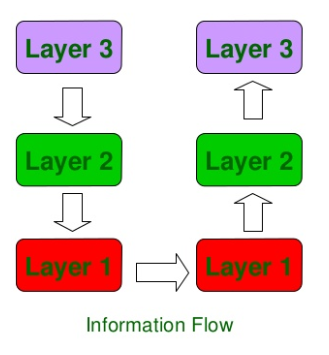
\includegraphics[scale=0.6]{24.png}
	\caption{Layer connections for GSM communication between 2 devices}
\end{figure} 

The network layer provides services to carry the message signal to its destination. The data link layer detects and resolves errors between the network layers of the 2 communicating devices. The physical layer i reponsible for transmission of the message signal on the physical medium. For example, a function like modulation for the transmission of data from the mobile station to the BTS occurs at the physical layer.

Each band is assigned a frequency by the GSM. This is known as Frequency Division Multiple Access.The size of each division is equal to 200 kHz.\\\\
The user's phone number on the service provider's network is known as the Mobile Subscriber ISDN. This is number is what is dialed by another subscriber to communicate with this subscriber. The MSISDN is split into  parts namely the Country Code represented by CC, the National Destination Code represented by NDC and the Subscriber Number represented by SN.\\
\begin{figure}[h]
	\centering
	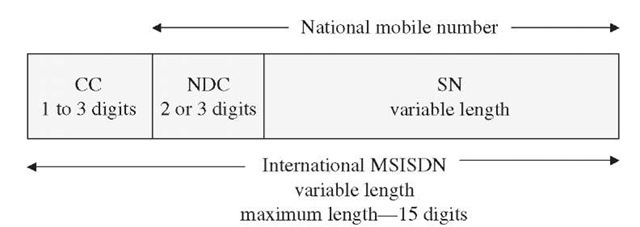
\includegraphics[scale=0.6]{20}
	\caption{MSISDN segments}
\end{figure}
\\
The CC is the international dialing code that the service provider of the subscriber is registered to. Each PLMN has its own NDC. The SN is the number that the user is registered as to the service provider. The concatenation of the NDC and the SN produces the National Mobile Number which is also known as the Local Mobile Number. This number is the nummber dialed by other subscribers in the same country as thee current user's service provider.\\
\begin{figure}[h]
	\centering
	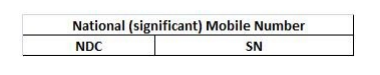
\includegraphics[scale=0.8]{21}
	\caption{National Mobile Number segments}
\end{figure}
\\
An example of a network provided by a service provider is the PLMN. The Mobile Station is subdivided into two modules: the Mobile Equipment represented by ME and the SIM.
\\
\begin{figure}[h]
	\centering
	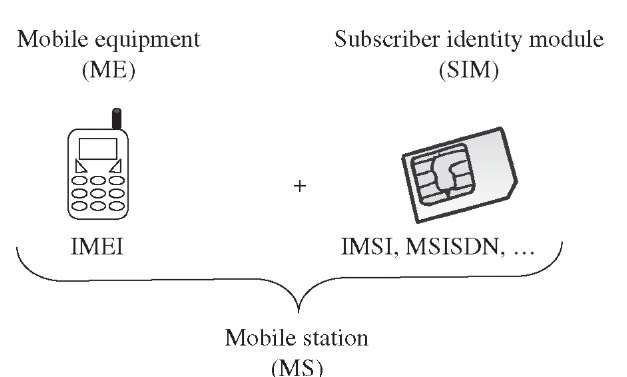
\includegraphics[scale=0.8]{22}
	\caption{A set-up of a Mobile Station}
\end{figure}
\\
As shown in the Figure 23, the ME is the physical component of the mobile station which is the cell phone. The primary requirement is that the phone should operate and communicate with other devices in a GSM network. The number of frequency bands that phones are operational in has increased from single to double to triple and finally to the modern phone which is quad-band. These phones have universal functionality in any GSM network. Each mobile handset has a unique International Mobile Equipment Identity printed onto it by the manufacturer.\\\\
The SIM is a very small card that should be inserted into the mobile phone for GSM connectivity. The card contains the subscriber's informations which includes their PIN code for access and the name of their service provider. The PIN code to access the SIM card is typically 4 digits long but if the code is entered wrongly for a certain amount of consecutive times depending on the service provider, the SIM cad is blocked. The user then has to enter an 8-digit PUK code to unblock the SIM card.

The model for the mobile station is adapted for the home shopping list device as well. Instead of the mobile equipment, the device can contain a GSM module integrated to the micro-controller that runs the shopping list device which is on the development board. The SIM card can then be placed inside the GSM module to form a fully functional mobile station.

The GSM network communicates with the mobile device or the shopping list device using a Base Transceiver Station. Multiple Base Transceiver Stations are controlled by a central Base Station Controller (BSC). The BSC also assigns radio frequencies from the mobile station.
\begin{figure}[h]
	\centering
	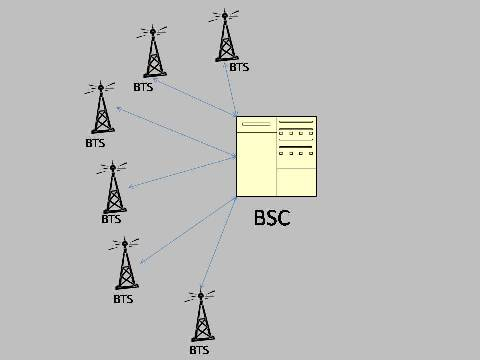
\includegraphics[scale=0.6]{23}
	\caption{BTS connections to a central BSC}
\end{figure}
\\
When the mobile station or the home shopping list device wants to access the GSM network, it goes through an authentication process which is normally at boot time, where the user has to prove their identity and be  permitted to use the network if they satisfy the authentication process. The authentication process is implemented by encryption. Cipher block design is used for development of the encryption algorithm. Some networks instead use convolutional coding for their encryption algorithms.

The central component of the GSM network is the Mobile Switching Center (MSC). The MSC handles the authentication process from the last paragraph. Calls are switched and mobile stations are granted roaming access using the Home Location Register (HLR) and the Visitor Location register. A mobile station's national mobile number is stored in the Equipment Identity Register (EIR) which has records of all mobile stations connected to the GSM network. The MSC can remotely access this EIR as can another MSC in a different mobile network.

Additionally a Short Message Service Centre is another component of the system and it stores holds transmitted messages into memory and sends them to the destination mobile stations. When a mobile station enters a different service provider's GSM network it can be granted access to services provided by this service provider at significantly higher than normal billing rates.

Interference is the most drawback associated with GSM communication. During a 2-way call, a user speaks for approximately half of the time as they spend approximately half of the time listening to the receiver[19]. Due to this property, the connection is made discontinuous leading to less power loss from each transmission. This works well for short message service as the communication does not need to be on all the time. 
 
Alternatively, Wi-Fi communication could be used. The theory associated with this communication method is discussed in the paragraphs that follow.
 
 
The IEEE 802.11 is the most widely used Wi-Fi standard. It is a standard of the Wireless Local Area Networks. The operating frequency bands of this protocol are typically $2.4$ GHz and $5$ GHz. The $5$ GHz spectrum provides more bandwidth, faster tranmsission speeds and higher reliability than the $2.4$ GHz frequency spectrum. Cell phones have undergone a gradual shift from circuit-switched networks ,which transmit data at peak speeds of 10 kbps to packet switched networks which transmit data at speeds of above 100 kbps. Wireless networks use packet switch for data transmission. The differences between packet switching and circuit switching are discussed in section 2.

WLAN was initially for operation in small-scale office rooms to avoid complex cabling in office computers. Therefore, most Wi-Fi systems extend to less than 200 m. The wireless networks can provide Internet access meaning communication is possible with devices beyond the radius as long as the sender is in the 200 m radius of the WLAN. Transmission speeds can go from 1 Mbps to as high as 10 Mbps [12]. 

What makes Wi-Fi more desirable than most communication models is that most modern devices come in with Wi-Fi functionality built-in just like GSM but the speed of transmission for WI-Fi is magnitudes of orders faster than GSM.

The basic topology of a Wi-Fi network is shown below.
\begin{figure}[h]
	\centering
	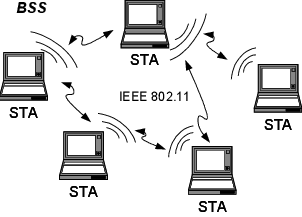
\includegraphics[scale=1]{25}
	\caption{Simple Wi-Fi topology for IBSS}
\end{figure}

For the above IBSS topology, the stations have peer-to-peer connections with each other and are called ad-hoc networks due to temporary connection style associated with the stations. These networks are very cheap and useful for tasks like conference meetings where user PCs only need connectivity with each other for a limited amount of time. This topology is extremely range limited. 

Multiple Basic Service Set topologies can be connected together by means of a distribution system to form an Extended Service Set topology. 
\begin{figure}[h]
	\centering
	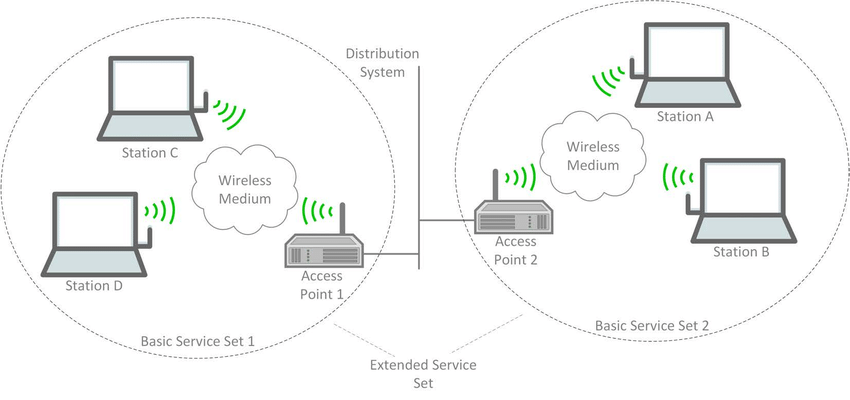
\includegraphics[scale=0.5]{26}
	\caption{Wi-Fi topology for ESS}
\end{figure}

The DS for the topology is usually any wireless network or Ethernet local area  network. The ESS enables the stations in different BSS networks to communicate with each other. The range available to ESS networks is significantly larger than the one provided by a single BSS topology. ESS is typically the design topology associated with Wi-Fi that covers entire university campuses.

The Access Point acts as a hub for wireless capable devices to communicate in the wireless LAN. The AP also authenticates devices that intend to devices that wish to communicate via the wireless network. The AP acts as the base station for PCs in the network. It also ports wireless networks together. A NIC is used by a a device with Wi-Fi capability for connectivity to the wireless network. The range of WLANs can be extended to kilometres by bridging LANs that are close to each other.


For the design of the Wi-Fi system, 3 design layouts were analyzed. A peer-to-peer wireless communication is when devices with NICs communicate directly with each other with no requirement for a server. The biggest problem with this layout is the range limit so a shopping list device with a NIC can only establish peer to peer connection with a user's phone when both devices are in the same residential range. Another layout is the Client and AP layout. The AP is connected to the service provider which offers server resources to the connecting PCs while extending their range of communication. The third layout is the Multiple AP layout. This is similar to the ESS topology where multiple APs are situated at different sites and they connect with each other to extend wireless coverage while giving wireless access to devices within their range.

A number of design limiting factors were analyzed for Wi-Fi. A device may have difficulty connecting to another AP in the ESS network. This can be due to to the connection not being therefore propagation delays being introduced and noise being introduced to the system through issues like interference. Peer to peer WLANs should only be used if the purpose is for the two device in the BSS to exclusively communicate with each other temporarily. The multiple AP WLANs should be used for devices who intend to access the Internet. The intended connection between the shopping list and the user's phone may use e-mail service for the shopping list device to receive a command to send the text and respond to the command with an email containing the text file. The use of the e-mail service implies the use of Internet therefore a multiple AP WLAN probably has to be implemented. However, peer-to-peer topology is used for the initial implementation of the WLAN. 

The interference of the WLAN can be due to other devices using frequency bands in the range similar to the one used for the WLANs i.e. $2.4$ GHz and $5$ GHz.  An example is the $2.4$ GHz 1EEE standard which competes with microwaves for frequency spectrum [22]. Due to this risk of interference, it is important for the information transmitted in the WLAN to be secured. Another big trade-off is that of battery life and bandwidth. The primary desire is data transmittion at high bandwidth but this leads to high battery drain for the Wi-Fi host. Therefore, for the home shopping list device an optimal frequency band has to be chosen so that battery drain is tolerable but not exponentially fast.  

The IEEE standard consists of 2 layers. These are Physical layer and the Media Acess control layer. The Physical layer consists of the frequency technology that is supported by the standard. These technolologies are frequency hopping, infrared and DS. Infrared technology is useful in BSS adhoc networks while microwave WLANs are used for multiple AP WLANs. DS WLANs need low traffic and transmit data at high data rates. The MAC layer is responsible for  the connection of the client device to the APs available. MAC also deals with the security of the WLAN.

The IEEE standards are split into 9 unique standards. The trade-off of interference for each standard is explored to choose the most applicable design. The important standards of note are:
\begin{itemize}
	\item 1EEE 802.11a : It is a physical layer standard which uses OFDM and priority is assigned to unique types of network traffic. The most important property is the low chance of interference due to operation in the $5$ GHz band. Transmission rates can be as high as 54 Mbps.
	\item IEEE 802.11b: Unlike the 802.11b standard, it operates in the $2.4$ GHz band and transmission speeds vary from 1 Mbps to 11 Mbps. Although the standard is old, other standards are just updates of this version with a few tweaks. The operation in the $2.4$ GHz band makes the standard susceptible to interference from other devices that operate in this frequency spectrum.
	\item IEEE 802.11c: This standard is important when designing and implementing access points so that APs can be bridged to extend WLAN coverage range.
	\item IEEE 802.11e: This standard is more dedicated to quality of service distribution for specific wireless local area networks. The standard focuses on the MAC layer to try to prioritize network traffic. Most of the priority is aimed at giving video and audio streaming services higher priority than the rest of the traffic. 
	\item IEEE 802.11f: When a Wi-Fi device switches between networks therefore switching to roaming mode, transmission packets are normally dropped and this standards atteempts to minimize the packets lost during handoffs when switching networks. Packets could also be dropped if an AP switches off due to some error and the device has to look for another AP in the multiple WLAN topology. 
	\item  IEEE 802.11g: The standard is backwards compatible with the 802.11b standard. It extends the transmission data rate of this protocol to be as high as 54 Mbps. Like the 802.11b standard,, the $2.4$ GHz band means the network is susceptible to interference as well.  
	\item IEEE 802.11i: This staandard focuses on the secure transfer of data on the network. All the other standards have weak security and this standard uses encryption for encryption schemes like AES to provide the best possible security.
\end{itemize}

Two stages are associated with each WLAN. These stages are authentication and encryption.
Authentication verifies if the client seeking communication is allowed to communicate with the server. Authentication can be provided by use of digital signatures or a pre-shared key.
The client has to prove they are who they claim to be. Encryption ensures secure data transfer between the two stations i.e. the user's phone and the home shopping list device. The data transferred over a wireless LAN can be susceptible to eavesdropping from hackers and the information transmitted can be compromised or worse, mal-ware can be attached to the file being transmitted. Examples of encryption schemes are Wired Equivalent Privacy and Wi-Fi Protected Access. WEP uses the same key at the client and the server for encryption and decryption.

The secure data transfer has to follow the stages shown in the diagram that follows.\\

\begin{figure}[h]
	\centering
	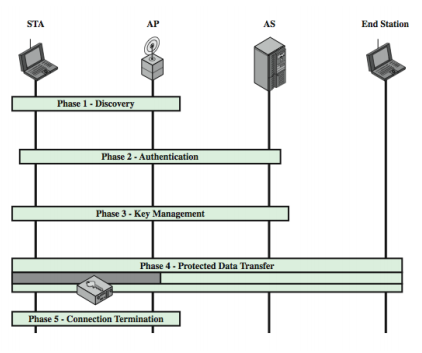
\includegraphics[scale=1]{28}
	\caption{Phases of operation for secure data transfer}
\end{figure}

The discovery phase involves the station and the access point identifying each other. The AP advertises its protocol using probe responses and the station detects them establishing an association between the two [17]. The authentication phase requires the station and the Authentication Server prove they are who they are to each other. Any data which is not for authentication is temporarily block from transmission in this phase. Cryptographic key generation is the next step in the phases shown and in the phase, the receiving stations receive these keys. If the communication is from one station to another via the use of an access point, like will be the case for the home shopping list to the user's phone, the keys will be group keys. If alternatively, the programmer intends to save the shopping list on the cloud which is on the Internet, then a pairwise key is generated for the AP. The two stations communicating can then exchange information between each other through the use of frames. Security is only applie to the station connection to the access point. Internet security can be implemented by using protocols like Secure Socket Layer protocol. E-mail already operates with SSL. After data exchange, the connection is terminated.

The comparison was also made between Wi-Fi and other wireless alternatives. Bluetooth transmission rates peak at  $\approx 800$ kpbs while Wi-Fi transmits at a significantly higher rate of $\approx 11$ Mbps. This project focuses on fast file transfer, therefore Wi-Fi is the more applicable choice for acceptable transmission times. If instead 3G communication is the alternative, then the decision for the right choice is a bit more close. The transmission speeds are a bit more closer as both schemes peak at $\approx 11$ Mbps. Wi-Fi is more design oriented for data transfer while 3G is an extension of the GSM communication with faster transfer rates. 

The home shopping device will be designed from different components with a development board. Most development boards are delivered with internal Wi-Fi modules while 3G modules have to purchased off the shelf and are fairly expensive. The 3G modules also have to be integrated onto the hardware which leads to either more wiring involved in the device if vero-boards are used or the device becoming larger in size which contradicts the requirement of the device being small-scale. Therefore for this project, Wi-Fi communication makes more sense to use as the data transmission method. 

\subsection{Modelling}

The handwriting writing and conversion process can be summarized by the flow chart below. The flow chart only documents the process from where the user writes onto the touchscreen until the user finishes writing onto the touchscreen.
\clearpage
\begin{figure}[h]
	\centering
	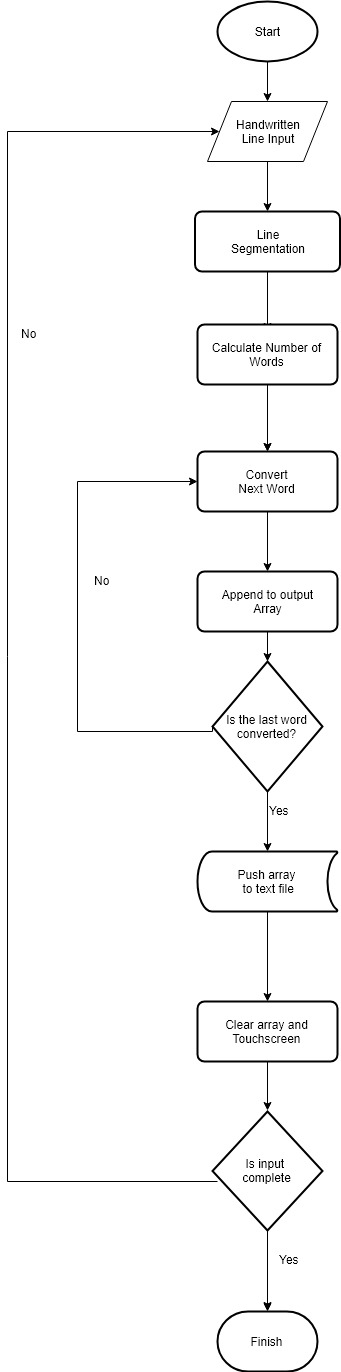
\includegraphics[scale=0.5]{34}
	\caption{Flowchart of the handwriting recognition process}
\end{figure}
\clearpage

A summary of the flow diagram is described. The user entered their shopping list line item onto the touchscreen. This input could be a sentence like "1 loaf of bread". The line input was only be restricted to one sentence per time and the sentence needed to be aligned on the touchscreen to reduce the skew. A line segmentation algorithm was applied to the input line so that the different words in the line could be obtained. In the sentence with, "1 loaf of bread", the words output after the line segmentation algorithm were "1", "loaf", "of" and "bread" separately. The number of these words was counted and the first word was converted. The converted output was pushed onto a string array. The word counter was reduced after successful word conversion and the word counter was checked if it was 0. If not, the next word was converted. After successful conversion, the output was appended with a space character between the initially converted word and the newly converted word. The word counter was decremented. The conversion process and appending the output onto an array was repeated until all the words from the line segmentation algorithm were completely converted. 

The output array after full conversion was then pushed to a text file and a new line was appended to the end of the text file sentence. The array containing the converted full word was then cleared to deallocate memory and the touchscreen was also cleared to provide input space for the net input. A button was made available for the user to indicate if they finished their input process.

Next, the shopping list from the conversion process had to be sent to the user's phone. The file had to be sent only when the user requested for it via e-mail. The flow chart on the next page details the steps that were taken for the file to be sent to the user's e-mail address. First, the Wi-Fi connection had to be established for the shopping list device to have an Internet connection. When an Internet connection had been established, the shopping list device would access the e-mail address assigned to it by default during the implementation process. The shopping list device would listen for a connection from the user's email address which was programmed within the communication algorithm. This process was generally known as the shopping device acting as the communicating server between the two devices, waiting for the client connection from the user's e-mail. When the user sent the e-mail, the sending process would be activated. The server was programmed to listen to any command from the user's email and this would trigger the process of sending the shopping list in the text file. The text file contents were read and stored  in an array of strings. The array of strings was then concatenated into a single string with elements separated by the newline character. The concatenated string was then sent to the user's email that had sent the command for the shopping list. The user then received the shopping list on their phone and did their shopping.
\clearpage
\begin{figure}[h]
	\centering
	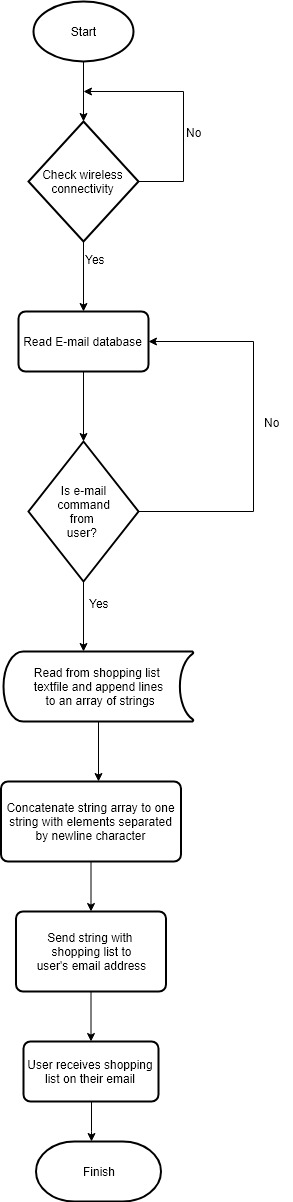
\includegraphics[scale=0.5]{36.jpg}
	\caption{Flowchart of sending the shopping list to the user's e-mail}
\end{figure}
\clearpage
\subsection{Optimization}
For the GSM network option, the transfer speeds of GSM are $\approx$ 10 kbps. The file size of the shopping list text file "shopping.txt" was found to be 586 kB. Therefore, the transmission time for the file to the user's device discounting the propagation delay was calculated as:
\begin{align*}
	t &= \frac{\text{File size}}{\text{Transmission Speed}}\\
	&= \frac{586 \times 8 \times 10^3 bits}{10 \times 10^3 bits/s}\\
	&= 46.9\,s
\end{align*}

This is way very slow and does not meet the time specifications of the product.

A trade-off is analyzed for the frequency band for the Wi-Fi communication. The frequency band in important in determining the Wi-Fi module to use for the shopping list device. Infrared waves cannot penetrate walls therefore are extremely range limited but offer very fast transmission speeds. On the other hand, radio waves can travel long distances but their data transmission rates are significantly lower. The two properties can be quantitatively compared by taking an example of 20 km between the source and destination. This models a situation where the customer shops 20 km from their home and requests the shopping the list in a wireless manner. The calculations associated with this transmission are shown below.\\
\newpage
\subsection{Data Design}
The software process of the project was modulated into different components. The components were listed as follows:
\begin{itemize}
	\item[1.]	Handwriting Recognition Algorithm
	\item[2.]	Graphical User Interface
	\item[3.]	E-mail communication
\end{itemize}

\textbf{Handwriting Recognition Algorithm}\\
The handwriting recognition algorithm was programmed using the Python programming language. Alternatively, it could be programmed by using Java, but the ability of Python to do mathematical functions on vectors was of great importance to reduce time complexity compared to Java which applied calculations element by element.

\textbf{Graphical User Interface}\\
The Graphical User Interface was programmed using PyQt, which uses the Python programming language for Widget development. PyQt was used instead of Qt because Qt uses the C++ environment, which complicates the integration process with the rest of the software components.

\textbf{E-mail Communication}\\
The e-mail communication software component facilitated the shopping list device receiving commands to send the shopping list and responding with the shopping list. Python programming was used for programming due to the availability of the Simple Mail Transfer Protocol which could be used to develop an e-mail server.

\subsubsection{Internal Software Data Structure}
The characteristic of the recognition algorithm to learn and update weight components required the use of  dynamic arrays. This is due to the fact that memory could be deallocated easily when dynamic arrays were used. Additionally, a 2-dimensional array will be associated with the PyQt GUI widget.

\subsubsection{Global Software Data Structure}
The output from the handwriting recognition process was saved globally so that it could be used by the e-mail server to send the shopping list to the client's phone therefore the string data structure, which was used to save the handwriting converted output was a global variable. Alternatively the data structure could have been a character array. Additionally, the shopping list could be requested any time, even during data input therefore the boolean data structure for listening to an incoming email request was global. 
\subsubsection{Temporary Data Structure}
The data structures which were temporary were mainly found in the recognition process. The errors were calculated for each output neuron and summed up before calculating the derivative. The error array then needed to be deallocated from memory. Another temporary variable was the count which was used for counting the number of words in the input sentence. As soon as the whole input was fully converted, this variable had to be reset and cleared until the next handwriting input. This variable was an integer.

\subsubsection{Database Description}
\textbf{2D Array Name}: widget$\_$Display\\
\textbf{Attributes}: save$\_$input, clear$\_$screen, capturedImage\\
\textbf{Description}: The array saved the resolution coordinates of the touchscreen and their colours. Initially, these were all zero values which represented the blank white screen. This database was important for the saving of user input by entering the non-white components of the touchscreen to their corresponding coordinates in the 2 dimensional array. The array contained integer values of  and 0, with 0 representing white and 1 representing non-white points from the screen-shot stored in capturedImage. \\\\
\textbf{2D Character Array Name}: shoppingList\\
\textbf{Attributes}: neural$\_$out, widget$\_$Display\\
\textbf{Description}: This array stored the outputs from the neural network. The neural network outputs were first concatenated after learning and error correction and they were then passed through a Viterbi algorithm to determine the closest word in the user's custom dictionary. The words were then combined to get the full initially input sentence. This word was then passed to the next free row of this array $shoppingList$ so that each row contained a sentence that was converted from the written sentence on the touchscreen, which was provided form widget$\_$Display.  \\\\
\textbf{Stack Name}: email$\_$Inbox\\
\textbf{Attributes}: email$\_$address, new$\_$mail\\
\textbf{Description}: The device had to access its email inbox database, first checking if new mail was received since the last access by using  the variable new$\_$mail which was a boolean. New mail was saved onto the argument stack and read. If the mail was not relevant, then the new$\_$mail variable would just be cleared but if the mail was from the desired client, the communication algorithm would send the shopping list to the email address of the stack element. 

\subsection{Architectural and Component Level Design}
\subsubsection{Program Description}
The structure chart method was used to represent the architectural diagram for the shopping list device. The dotted connections showed the partial dependencies of the architectural blocks connected. The classes that were designed to include the component block used the hierarchal class structure to show the most important classes for the device to be operational.
\subsubsection{Architecture Diagram}
The architectural block diagram of the home shopping list device software was shown below.
\begin{figure}[h]
	\centering
	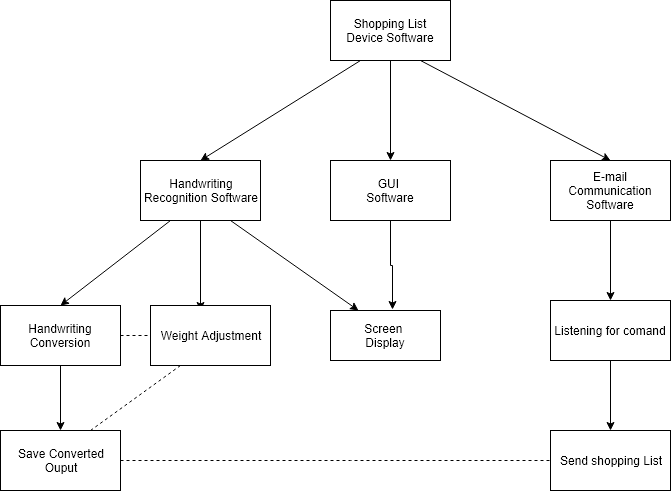
\includegraphics[scale=0.6]{38}
	\caption{Architectural diagram for the shopping list device}
\end{figure}

\subsubsection{Architectural Component Description}
The software component of the device was divided into 3 classes which were designed as shown in the figure that follows.
\begin{figure}[h]
	\centering
	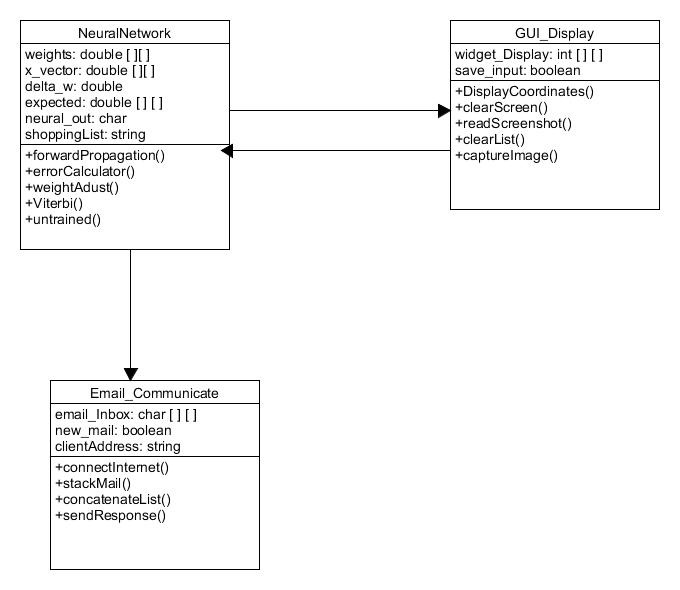
\includegraphics[scale=0.6]{42}
	\caption{Architectural diagram for the shopping list device}
\end{figure}

\subsubsection{Description of Components}
\textbf{Component NeuralNetwork}
\begin{itemize}
	\item \textbf{Processing Narrative of NeuralNetwork}: The attributes of the component include the weight matrix which was randomly generated, the input values from the touchscreen screen-shot, the character output after a neural network conversion and the full converted word. This was the most important component of the  home shopping list device's software because without it, no conversion would to take place thus the device would only contain handwritten screen-shots.
	\item \textbf{Interface Description of component NeuralNetwork}: The component interfaced with the GUI$\_$Display to get the vector representation of the 2D $x-$input array. It also saved the full word output to the full shopping list array which it passed to the communication component on request.
	\item \textbf{Algorithmic Description of the NeuralNetwork component}: The component links all three components of the software system as follows:\\
	\begin{itemize}
		\item[$\diamond$]	START
		\item[$\diamond$]	Get $\vec{x}$ from component GUI$\_$Display
		\item[$\diamond$]	Convert the full input sentence and store.
		\item[$\diamond$]	Listen for connection from Email$\_$Communicate and send the stored sentence. 
	\end{itemize}
\end{itemize}
The pseudocode for this component's most important function of handwriting recognition is shown below:
\begin{algorithmic}
	\STATE $\vec{x}$ $\Leftarrow$ GUI$\_$Procedure.widget$\_$Display 
	\STATE $\vec{w} \leftarrow$ \textbf{random}(length($\vec{x}$)) $\hfill \rightarrow$ Randommly generated weight array
	\STATE $x_{bias} = 1$  $\hfill \rightarrow$ Initialize bias neuron
	\STATE $w_{bias} = \textbf{random}$ $\hfill$ Generate weight of bias neuron
	\STATE $net_j = 0$ $\hfill$ Initialize neuron output
	\FOR {every neuron in every layer}
	\FOR {i in range length($\vec{x}$)}
		\STATE $net_j += \vec{x}\cdot vec{w}$
	\ENDFOR
	\STATE $net_j += x_{bias}\cdot w_{bias}$
	\STATE $a_j \leftarrow \frac{1}{1+e^{-net_j}}$
	\STATE $neuron_{out} \leftarrow a_j$
	\STATE $layer_out$ $\Leftarrow$ $neuron_out$
	\STATE Update $\vec{x}$ for next layer to consider $layer_{out}$
	\ENDFOR
	\IF {layer = outputLayer}
	\STATE$\sigma_s = neuron_{out} - e_j$ $\hfill$ Compare output to expected.
	\STATE $\Delta w = \sigma_s \cdot neuron_{out}$
	\WHILE {d ($\sigma_s$) $\neq 0$}
	\STATE $\vec{w} = \vec{w} - \Delta w$
	\STATE $net_j = \sum{\vec{w} \cdot \vec{x}} + 1\cdot (w_{bias})$
	\STATE$\sigma_s = neuron_{out} - e_j$  
	\ENDWHILE
		\STATE $output \leftarrow \frac{1}{1+e^{-net_j}}$
	\ENDIF
\end{algorithmic}

\textbf{Design  Class Hierarchy}\\
\begin{figure}[h]
	\centering
	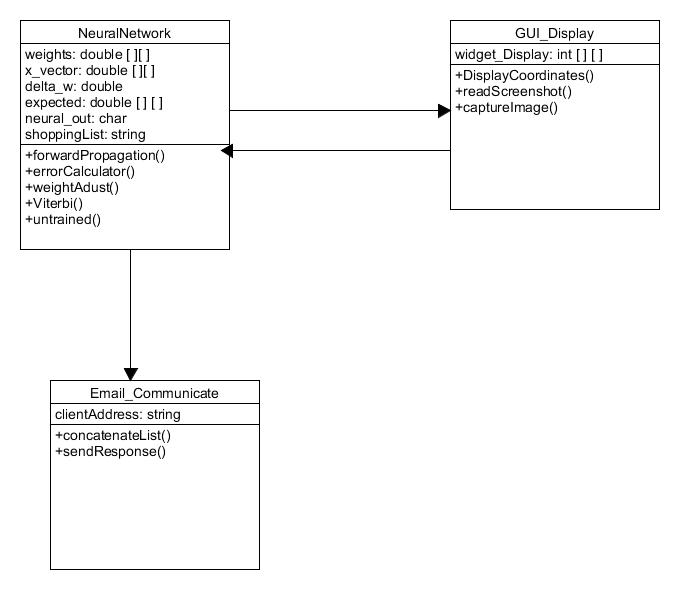
\includegraphics[scale=0.5]{41.jpg}
	\caption{Design class hierarchy for NeuralNetwork component}
\end{figure}

The design class hierarchy shows the specific functions from the connected functions that interact with the component.

\textbf{Restrictions}\\
 The number of hidden layers chosen had to be enough for significant accurate recognition but not too much because too much time would have been spent back-propagating and correcting errors.

\textbf{Component GUI$\_$Display}
\begin{itemize}
	\item \textbf{Processing Narrative of GUI$\_$Display}: The attributes in the component included the 2D array to save the equivalent screen inputs and a button which could clear the touchscreen when pressed.
	\item \textbf{Interface description of GUI$\_$Display}: The component interfaced with the NeuralNetwork component to provide the necessary vector array of inputs after converting the screen shot from the touchscreen to integer values in the array.
	\item \textbf{Algorithm Description of the GUI$\_$Display} : The link between the two components can be described in short as follows:
	\begin{itemize}
		\item[$\diamond$] START
		\item[$\diamond$] Prompt handwriting input
		\item[$\diamond$] Save Image of User Input
		\item[$\diamond$] Map the image coordinates to the 2D array of inputs.
	\end{itemize}
\end{itemize}
The pseudocode associated with the screen capturing and saving part is shown below:

\begin{algorithmic}
	\STATE widget$\_$Display = \textbf{empty}([] []) $\hfill$ Initialize empty GUI screen 
	\STATE coordinatesPen = [0,0] $\hfill$ Initialize mouse/pen drawing tool to null
	\IF {user enters drawing on screen}
	\WHILE {finishedDrawing $==$ \textbf{false}}
	\STATE draw += coordinatesPen $\hfill$ Take user's pen input.
	\ENDWHILE
	\STATE drawnImage = draw $\hfill$ The summed up user pen drawings.
	
	
	\textbf {for} {[\textbf{row}(drawnImage),\textbf{column}(drawnImage)]}  \textbf{do}
	\IF {drawnImage[row, column] == white}
	\STATE $widget\_Display$ [row, column] = 0
	\ELSE
	\STATE $widget\_Display$ [row, column] = 1
	\ENDIF
	
	\textbf{end for}
	%\ENDFOR
	
	\ENDIF 
\end{algorithmic}
	
\textbf{Design class hierarchy}
The design class hierarchy diagram shows the functions used by the NeuralNetwork component that interfaces with the GUI$\_$Display component.

\begin{figure}[h]
	\centering
	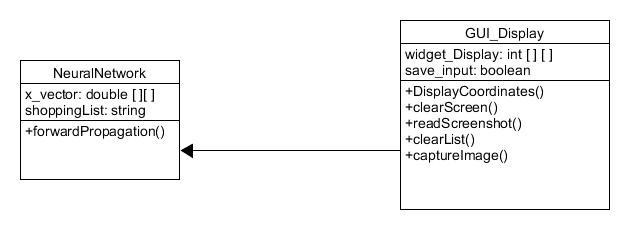
\includegraphics[scale=0.6]{43.jpg}
	\caption{Design class hierarchy for GUI$\_$Display component}
\end{figure}

\textbf{Restrictions}\\
The pen drawing application had a trade-off of fine ink which produced dots which overlapped against the pixel array but drawn characters were easily recognizable and sharp ink which produced the pen input images into different pixels but the image detection of the colours sometimes wrongly detected blank inputs due to the pixel most being white but containing a fraction of black ink.

\textbf{Component Email$\_$Communicate}
\begin{itemize}
	\item \textbf{Processing Narrative of Email$\_$Communicate}: The attributes in the component included the variable to check for new mail, the stack of inbox mail and the email address of the client
	\item  \textbf{Interface description of Email$\_$Communicate}: The component interfaced with the NeuralNetwork component to save the converted sentence into a string and store it as a text file offline. The file's contents would then be sent to the user's email address on request.
	\item \textbf{Algorithm Description of Email$\_$Communicate}: The tasks in volved in the component were shown procedurally as follows:
		\begin{itemize}
		\item[$\diamond$] START
		\item[$\diamond$] Update shopping list with new converted sentence.
		\item[$\diamond$] Check new mail and update onto mail stack.
		\item[$\diamond$] Check address of new mail.
		\item[$\diamond$] Send shopping list contents if the new mail email address is the same as the client address.
	\end{itemize}
\end{itemize}

\subsection{Design summary}
\begin{center}
	\begin{longtable}{|p{4cm}|p{7cm}|p{5cm}|}
		\hline 
		\textbf{Task} &
		\textbf{Implementation} &
		\textbf{Task Completion}
		\\
		\hline
		Design of non-USB battery system& The off the shelf 5 V battery was bought off the shelf. The Raspberry Pi's touchscreen and the Raspberry Pi were connected to it & Complete\\
		\hline
		&  &  \\
		\hline
		 &  & \\
		
		\hline
		\caption{Design summary.}
	\end{longtable}
\end{center}
\newpage

%% End of File.

